%!TEX program = xelatex

%% 版本:1.0
%% 2022-05-07
%% 作者:杨永全
\documentclass[aspectratio=169,UTF8,t]{beamer}%比例是16:9,UTF8编码支持,顶部对齐
\usepackage{oucslide}
\usepackage[UTF8]{ctex}
\usepackage{xeCJK}
\usepackage{fontawesome}%加入图标支持
\usepackage{tcolorbox}
\usepackage{verbatim}
\usepackage{caption}
\usepackage{subcaption}

\newcommand\crule[3][black]{\textcolor{#1}{\rule{#2}{#3}}}

%基本信息
\title{中国海洋大学幻灯片Latex模板}
\subtitle{助力你的科研梦想}
\author{杨永全}
\date{\today}
\institute{计算机科学与技术学院}
\newcommand{\last}{敬请批评指正!} %结束语
%\newcommand{\last}{提问与解答环节}
%基本信息结束

\begin{document}

\maketitle

\makeoutline

\section{简介}

\subsection{模板简介}

\begin{frame}
    \frametitle{简介}
    中国海洋大学演示文稿Latex非官方模板。

    本模板修改自HelmholtzAI\footnote{https://github.com/Helmholtz-AI-Energy/beamer-template}模板。在原有模板基础上进行了大量修改。

    模板主要使用海大公布的标准色,包括海大蓝、海大天蓝、海大红、樱缤粉、文脉棕、专金、专银。

    此外,使用了大量的信息框来增加模板的活力。
    \begin{center}
        \begin{figure}
        \centering
        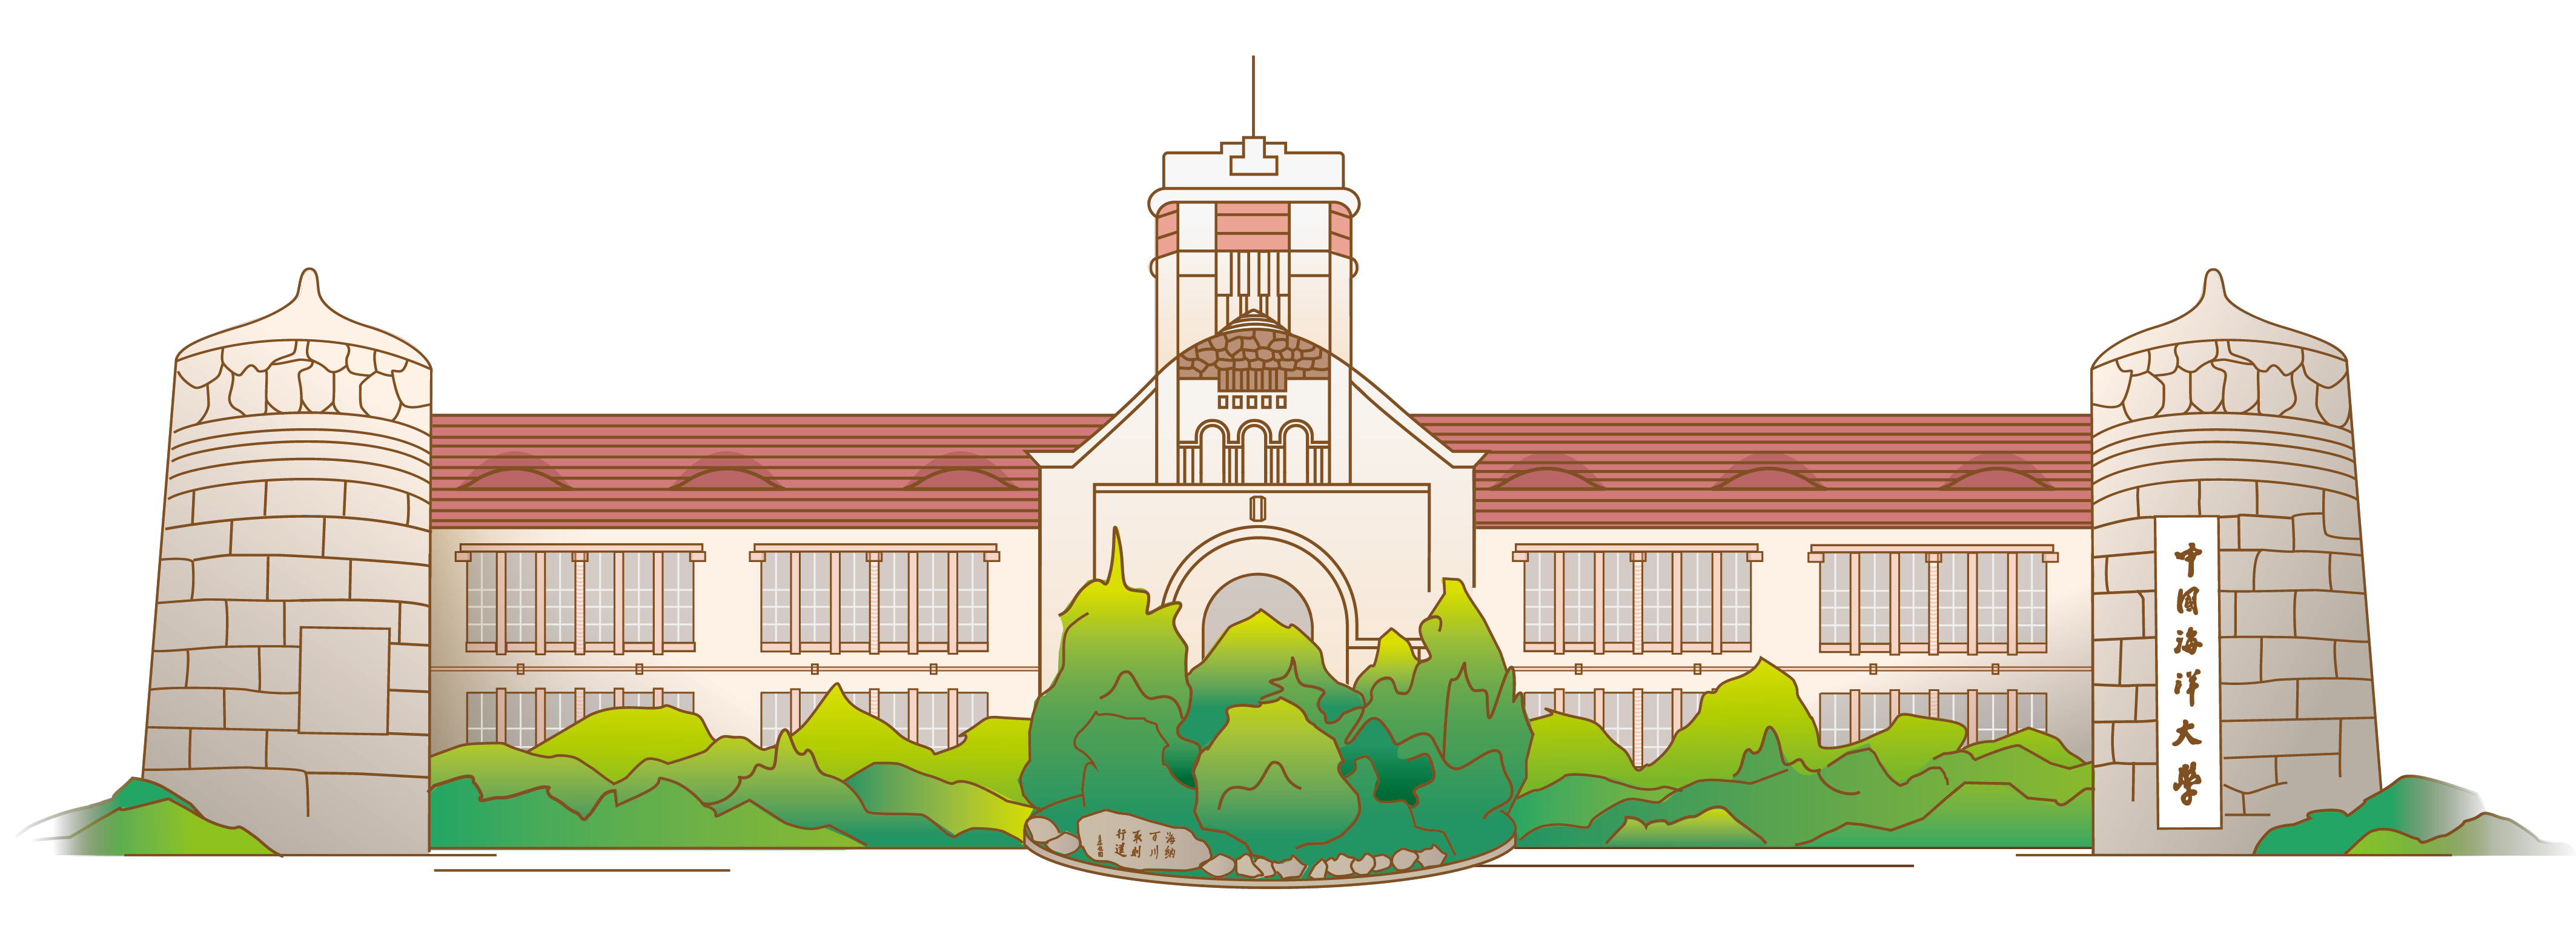
\includegraphics[width=0.6\textwidth]{figs/ouc.png}
            \caption{中国海洋大学}
            \label{fig:ouc}
        \end{figure}
    \end{center}
    
    
\end{frame}

\section{模板使用方法}

\subsection{使用方法}

\begin{frame}
    \frametitle{模板使用方法}    
    \begin{enumerate}
        \item 从git上clone整个文件夹目录\footnote{https://git.yangyq.net/laoyang/ouc-slide-latex-template.git }\footnote{https://github.com/dryangyq/ouc-slide-latex-template.git}\footnote{https://gitee.com/dryangyq/ouc-slide-latex-template.git}\footnote{https://gitlab.com/dryangyq/ouc-slide-latex-template.git}\\~
        \item 编辑tex文件进行修改\\~
        \item 编译tex文件为PDF\\~
        \begin{enumerate}
            \item 可以使用VS Code,或者\\~
            \item 使用LaTeX IDE,比如TeXstudio等进行编译\\~
        \end{enumerate}
        \item \emph{注意:} 请使用LuaLaTeX 或者 XeLaTeX 进行编译
    \end{enumerate}
\end{frame}

\section{元素}

\subsection{字体}

\begin{frame}
    \frametitle{字体是啥}
    模板使用的默认字体是鸿蒙字体。

    如果对字体不满意,可下载其他字体,放入fonts文件夹,并在\textbf{beamerfontthemeOUCSlide.sty}文件中修改。
    \begin{center}
        \begin{figure}
        \centering
        
\includegraphics[width=0.5\textwidth]{figs/harmonysans.png}
            \caption{鸿蒙字体}
            \label{fig:harmonysans}
        \end{figure}
    \end{center}
\end{frame}

\subsection{颜色}
\subsubsection{基本颜色}
\begin{frame}
    \frametitle{颜色}
    %\framesubtitle{基本颜色}
    
    根据海大公布的标准颜色,定义了相关颜色,主要包括海大蓝、海大天蓝、海大红、樱缤粉、文脉棕、专金、专银。其中文名称和代码如表\ref{table:color}所示。\\
    当然,也可以使用Latex自带的颜色,例如white、black等。
    
    \begin{table}
        \centering
        \small
        \caption{基本颜色定义}
        \label{table:color}
        \begin{tabular}{ccc}
            \textbf{颜色} & \textbf{名称} & \textbf{中文名}\\\toprule
            \crule[oucblue]{10pt}{10pt} & oucblue & 海大蓝 \\
            \crule[ouclightblue]{10pt}{10pt} & ouclightblue & 海大天蓝 \\
            \crule[oucred]{10pt}{10pt} & oucred & 海大红 \\
            \crule[ouccherry]{10pt}{10pt} & ouccherry & 樱缤粉 \\
            \crule[oucbrown]{10pt}{10pt} & oucbrown & 文脉棕 \\
            \crule[oucgolden]{10pt}{10pt} & oucgolden & 专金 \\
            \crule[oucsilver]{10pt}{10pt} & oucsilver & 专银 \\
        \end{tabular}
    \end{table}
\end{frame}

\subsubsection{颜色等级}

\begin{frame}
    \frametitle{颜色}
    %\framesubtitle{颜色等级}
    
    \emph{定义的海大标准色,每一种颜色,都有十个等级,等级越低,颜色越浅。例如:对于海大蓝,其等级颜色如表\ref{table:colorgrade}所示。}\\
    
    \begin{table}
        \centering
        \small
        \caption{颜色等级}
        \label{table:colorgrade}
        \begin{tabular}{cl}
            \textbf{颜色} & \textbf{名称}\\\toprule
            \crule[oucblue10]{8pt}{8pt} & oucblue10 \\
            \crule[oucblue20]{8pt}{8pt} & oucblue20 \\
            \crule[oucblue30]{8pt}{8pt} & oucblue30 \\
            \crule[oucblue40]{8pt}{8pt} & oucblue40 \\
            \crule[oucblue50]{8pt}{8pt} & oucblue50 \\
            \crule[oucblue60]{8pt}{8pt} & oucblue60 \\
            \crule[oucblue70]{8pt}{8pt} & oucblue70 \\
            \crule[oucblue80]{8pt}{8pt} & oucblue80 \\
            \crule[oucblue90]{8pt}{8pt} & oucblue90 \\
            \crule[oucblue]{8pt}{8pt} & oucblue \\\bottomrule
        \end{tabular}
    \end{table}
\end{frame}

\subsection{副标题和列表}

\subsubsection{\textbf{副标题}:可以补充更多信息}

\begin{frame}
    \frametitle{副标题和列表}
    副标题,可以展示不同的层级关系,一般用来显示内部章节。\\
    幻灯片的标题,都使用section进行规划,内部的frametitle中的内容将不再起作用。一级标题,使用单独的幻灯片进行展示,并显示在目录幻灯片中。二级和三级标题,在幻灯片的标题部分进行显示,带有自动编号。\\
    可以使用内部列表展示幻灯片中的层级关系。这里是无序列表的样子。
    \begin{itemize}
        \item 这里展示一个列表 
        \item 列表可以是多级
        \begin{itemize}
            \item 这里是二级
            \begin{itemize}
                \item 这里是三级标题
            \end{itemize}
            \item 顺序是无所谓的
        \end{itemize}
    \end{itemize}
\end{frame}

\subsection{列表框}

\begin{frame}
    \frametitle{列表框}
    列表框一般用来展示列表内容,使用vcolorbox,可以使用自定义颜色。
    \begin{vcolorbox}[中国海洋大学]{oucred}
        1. 211、985重点高校

        2. 世界一流大学建设高校(A类)。
    \end{vcolorbox}
    \begin{vcolorbox}[学校校训]{ouclightblue}
        海纳百川,取则行远
    \end{vcolorbox}
    \begin{vcolorbox}[学校特色]{oucblue}
        1. 海洋和水产学科特色显著
        
        2. 学科门类齐全
    \end{vcolorbox}
\end{frame}

\subsection{提示框}

\begin{frame}
    \frametitle{提示框}
    提示框共两类,一类是笔记提示框(notebox),一般用来提示学生记录笔记;另外一类是重要信息提示框(importantbox),默认使用红色,具有更强的视觉冲击力。
      \begin{notebox}[笔记]
        请大家把这里的笔记记录下来,是重点内容。 
      \end{notebox}
      \begin{importantbox}[重要]
        考试时禁止任何形式的作弊行为!
      \end{importantbox}              
\end{frame}

\subsection{信息框}

\begin{frame}
    \frametitle{信息框}
    信息框(titlebox)主要用来勾勒一些需要注意的信息,颜色可以自定义。
    \begin{titlebox}[提示框]{oucred}
        这里展示的是海大红颜色的提示框。
      \end{titlebox}
      \begin{titlebox}[颜色展示]{oucblue}
        这里展示海大蓝的颜色。当然,可以使用更多的颜色。 
      \end{titlebox}
      \begin{titlebox}[另外一些颜色的显示]{ouclightblue}
        这里展示海大天蓝的颜色。当然,可以使用更多的颜色。 
      \end{titlebox}    
\end{frame}

\subsection{要点框}

\begin{frame}
    \frametitle{要点框}
    要点框(pointbox)主要用来展示一些要点,需要和分栏配合使用,颜色可以自定义。 \\   
    高度可以写在参数中。  
      \begin{columns}
        \begin{column}{0.3\textwidth}
            \begin{pointbox}[要点一]{oucred}{100pt}
                人文特色\\
                海洋特色\\                
            \end{pointbox}
        \end{column}
        \begin{column}{0.3\textwidth}
            \begin{pointbox}[要点二]{oucblue}{100pt}
                211\\
                985\\
                双一流 
            \end{pointbox}            
        \end{column}
        \begin{column}{0.3\textwidth}
            \begin{pointbox}[要点三]{ouclightblue}{100pt}
                院士\\
                杰青 
            \end{pointbox}
        \end{column}
    \end{columns}    
\end{frame}

\subsection{标题框和文本框}

\begin{frame}
    \frametitle{文本框}
    标题框和文本框配合使用,基本上可以满足大部分的内容展示需求。 \\       
    \begin{headbox}{oucred}
        中国海洋大学
    \end{headbox}  
    \begin{textbox}{oucblue}
        中国海洋大学是一所海洋和水产学科特色显著、学科门类齐全的教育部直属重点综合性大学,是国家“985工程”和“211工程”重点建设的高校,2017年9月入选国家“世界一流大学建设高校”(A类)。

        学校校训是“海纳百川,取则行远”。
    \end{textbox}
    \begin{textbox}{ouclightblue}
        学校创建于1924年,历经私立青岛大学、国立青岛大学、国立山东大学、山东大学等办学时期,于1959年发展成为山东海洋学院,1960年被国家确定为全国13所重点综合性大学之一,1988年更名为青岛海洋大学,2002年更名为中国海洋大学。
    \end{textbox}
      
\end{frame}

\subsection{块}

\begin{frame}
    \frametitle{块}
    块(block)共分为三种,分别是默认、example和alert,颜色分别使用海大蓝、专银和海大红。
    \begin{block}{默认块}
        一个系统默认的块,是这样的。
    \end{block}

    \begin{exampleblock}{例子}
        如果需要放入一些例子,可以用这个颜色的块。
    \end{exampleblock}

    \begin{alertblock}{提示块}
        这里展示的是需要额外注意的信息。
    \end{alertblock}
\end{frame}

\subsection{代码}

\begin{frame}[fragile]
    \frametitle{代码}
    
    请注意 [fragile] 这个关键字,是必须的。当然,也可使用定义好的另外一种frame,叫做fragileframe,他们的效果是一样的。该关键字的目的,是为了让代码保持它原有的样子。代码段的关键词是lstlisting。\\
    当前显示的效果还比较一般,后续将加入更多的颜色主题。

\begin{lstlisting}[language=Java,caption={src/app/app.module.ts}]
    import org.sun.com;   
    public class helloworld{
      public static void main()
      {
        System.out.println("hello world!");
      }
    }
    \end{lstlisting}
\end{frame}

\section{其他细节}

\subsection{公式}

\begin{frame}
\frametitle{公式}
    支持Latex原生的公式,当然也可以和文字进行混排。
    \begin{equation}
        f(x) = \sum_i wx_i^2 + \frac{\beta}{2} \label{eq:simple}  
    \end{equation}
    这里可以进行文字的说明,如式\eqref{eq:simple}所示。
\end{frame}

\subsection{栏目和图}

\begin{frame}
    \frametitle{栏目和图}

    \begin{columns}
        \begin{column}{0.4\textwidth}
            \begin{enumerate}
                \item 一个页面可以分为多栏\\~
                \item 栏目的宽度,需要自己进行定义\\~
                \item 可以导入图片\\~
                \item 可以根据情况对图片进行缩放
            \end{enumerate}
        \end{column}
        \begin{column}{0.4\textwidth}
            \centering
            \begin{figure}
                \centering
                
\includegraphics[width=\textwidth]{figs/ouc_gate.png}
                    \caption{中国海洋大学校门}
                    \label{fig1}
            \end{figure}
            
        \end{column}
    \end{columns}
\end{frame}

\subsection{脚注}

\begin{frame}
    \frametitle{脚注}
        可以在任何地方加入脚注,即便是在各种信息框\footnote{信息框包括:提示框、列表框、要点框等。}中也可以。
        \begin{notebox}[笔记]
            请大家把这里的笔记记录下来,是重点内容\footnote{考试要考。}。 
        \end{notebox}
\end{frame}

%最后一页
\makelast

\end{document}